\begin{figure}[h]
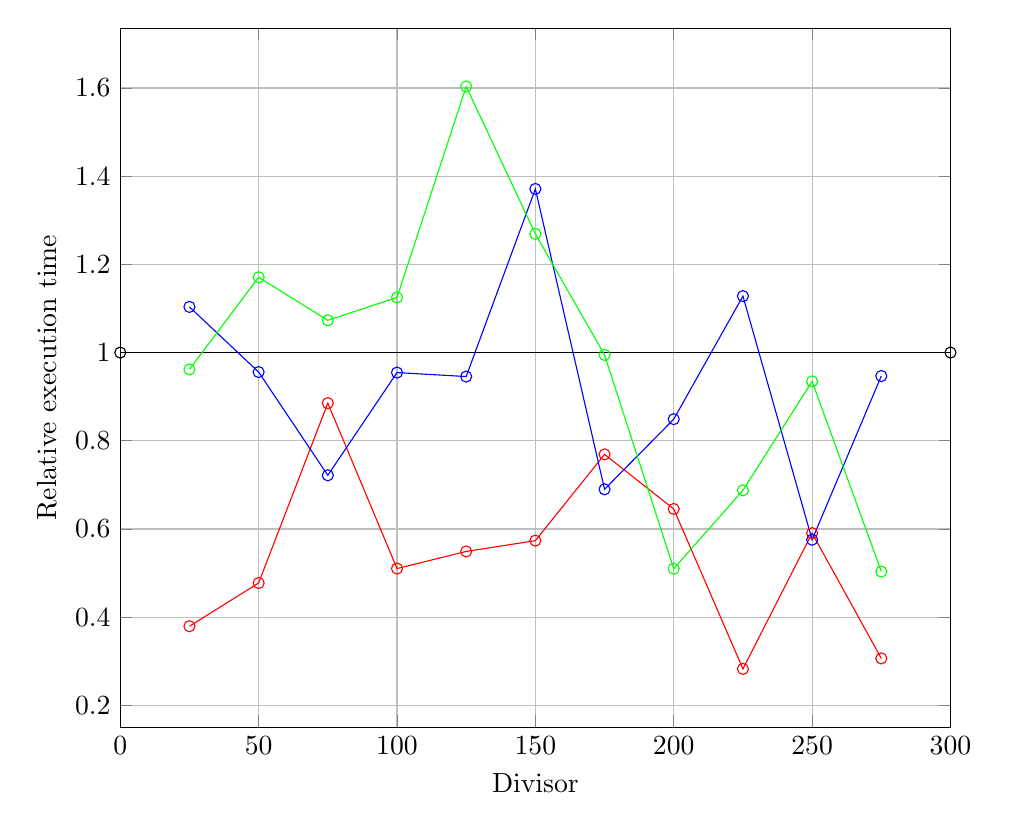
\begin{tikzpicture}
\begin{axis}[%
	grid=both,
	width=\textwidth,
	ylabel=Relative execution time,
	xlabel=Divisor,
	xmin=0,
	xmax=300,
	scatter/classes={%
    a={mark=o,draw=red}, 
    b={mark=o,draw=blue}, 
    c={mark=o,draw=green}, 
    d={mark=o,draw=black}}]
   
   
    \addplot[scatter,color=black,
    scatter src=explicit symbolic]%
table[meta=label] {
x y label
0 1  d
300 1   d
};
    
    %%% Instance 1
\addplot[scatter,color=red,%
    scatter src=explicit symbolic]%
table[meta=label] {
x y label
25 0.379421491422 a
50 0.477402260988 a
75 0.885413590617 a
100 0.510155923678 a
125 0.54898135615 a
150 0.573495346387 a
175 0.769136788114 a
200 0.64536373063 a
225 0.282592831425 a
250 0.590582666036 a
275 0.306450495165 a
};
    %%% Instance 2


\addplot[scatter,color=blue,%
    scatter src=explicit symbolic]%
table[meta=label] {
x y label
25 1.10355950744 b
50 0.955813425082 b
75 0.721665563736 b
100 0.954662492364 b
125 0.945632444074 b
150 1.37113745958 b
175 0.689947691066 b
200 0.848947873352 b
225 1.12809875303 b
250 0.575656154091 b
275 0.946829308358 b
};

%%% Instance 3
\addplot[scatter,color=green,%
    scatter src=explicit symbolic]%
table[meta=label] {
x y label
25 0.961924446699 c
50 1.17081862189 c
75 1.07323537789 c
100 1.12497429541 c
125 1.60348201399 c
150 1.26910123951 c
175 0.994641341841 c
200 0.509881892099 c
225 0.687597223698 c
250 0.934752079874 c
275 0.503438589419 c
};




       
\end{axis}
\end{tikzpicture}

\caption{Attempt at finding the best divisor for instances of size $N = 100$. Straight lines are results without adding the VI. The relative time is expressed as the ratio of the execution time with a given divisor over the reference execution time, without the VI. Dots represent the performance with various divisors. Instance \texttt{1.out} is in red, \texttt{2.out} in blue, \texttt{3.out} in green.}
\end{figure}